\documentclass{article}
\usepackage{hyperref}
\usepackage{float}
\usepackage[margin=1in]{geometry}
\usepackage[justification=centering]{caption}
\usepackage{amsmath,amsfonts,amsthm,fullpage,amssymb,algorithm,color,mathtools,float,hyperref,subcaption,url,graphicx, algorithmic}
\newcommand{\largeimagewidth}{350}
\newcommand{\mediumimagewidth}{250}

\begin{document}
\begin{titlepage}
\clearpage\thispagestyle{empty}
\centering
\vspace{1cm}

\rule{\linewidth}{1mm} \\[0.5cm]
{ \Large \bfseries ISYE 6740 - Fall 2023\\[0.2cm]
Final Project}\\[0.5cm]
\rule{\linewidth}{1mm} \\[1cm]

\begin{tabular}{l p{5cm}}
\textbf{Team Member Names:} William Luna (Solo) gtID: 903947280 &   \\[10pt]
\textbf{Project Title:} Speaker Attribution in Written Dialogue &  \\[10pt]
\end{tabular} 



\begin{figure}[H]
\centering
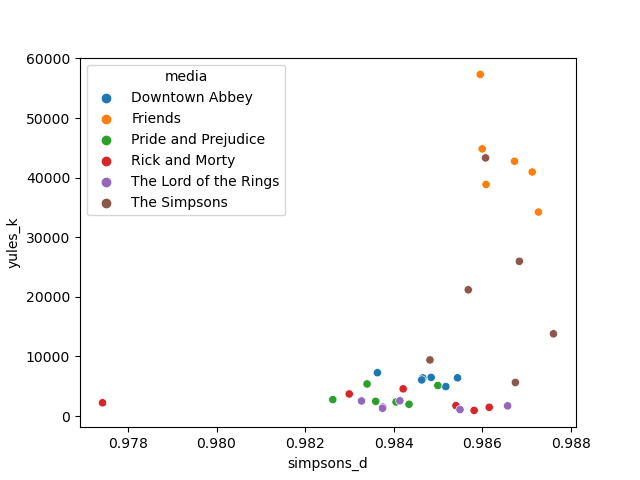
\includegraphics[width=\largeimagewidth]{images/heuristics.png}
\caption{Speakers within a piece of media tend to cluster together.}
\end{figure}

\begin{figure}[H]
\centering
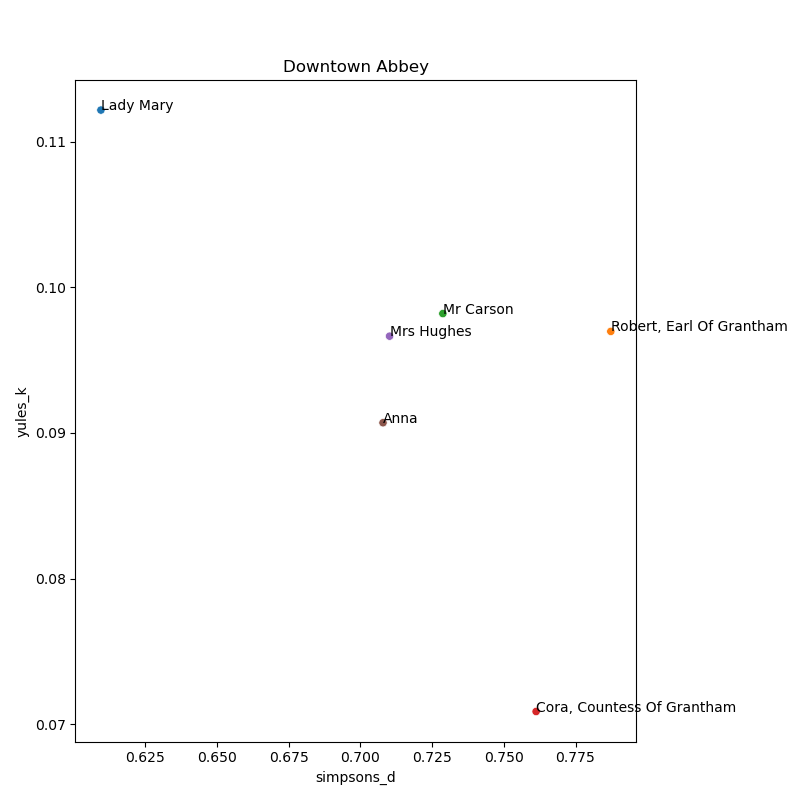
\includegraphics[width=\mediumimagewidth]{images/Downtown Abbey_heuristics.png}
\caption{Note that the three servants are clustered in the center while each member of the nobility occupies a distinct place in the plot.}
\end{figure}

\begin{figure}[H]
\centering
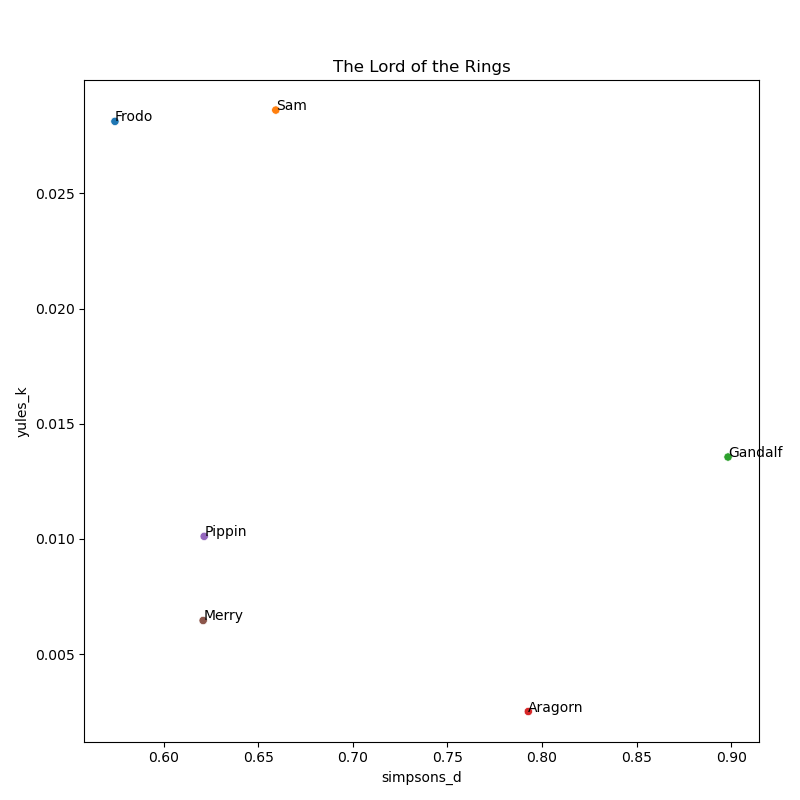
\includegraphics[width=\mediumimagewidth]{images/The Lord of the Rings_heuristics.png}
\caption{This scatter plot implies that Frodo and Sam have similar speech patterns, as do Pippin and Mary, distinct from Gandalf and Aragorn.}
\end{figure}

\begin{figure}[H]
\centering
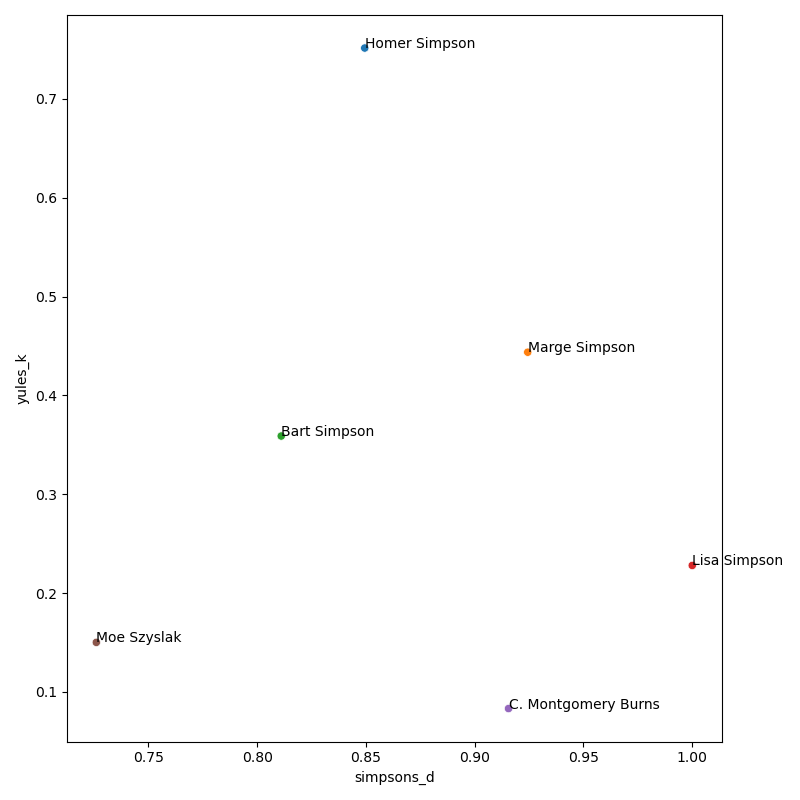
\includegraphics[width=\mediumimagewidth]{images/The Simpsons_heuristics.png}
\end{figure}

\begin{figure}[H]
\centering
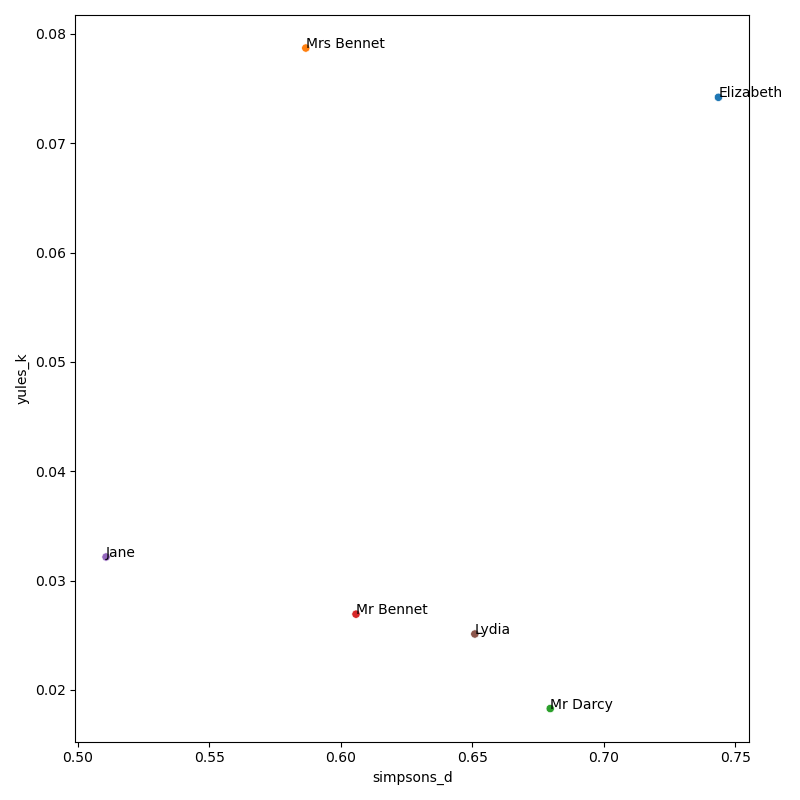
\includegraphics[width=\mediumimagewidth]{images/Pride and Prejudice_heuristics.png}
\end{figure}

\begin{figure}[H]
\centering
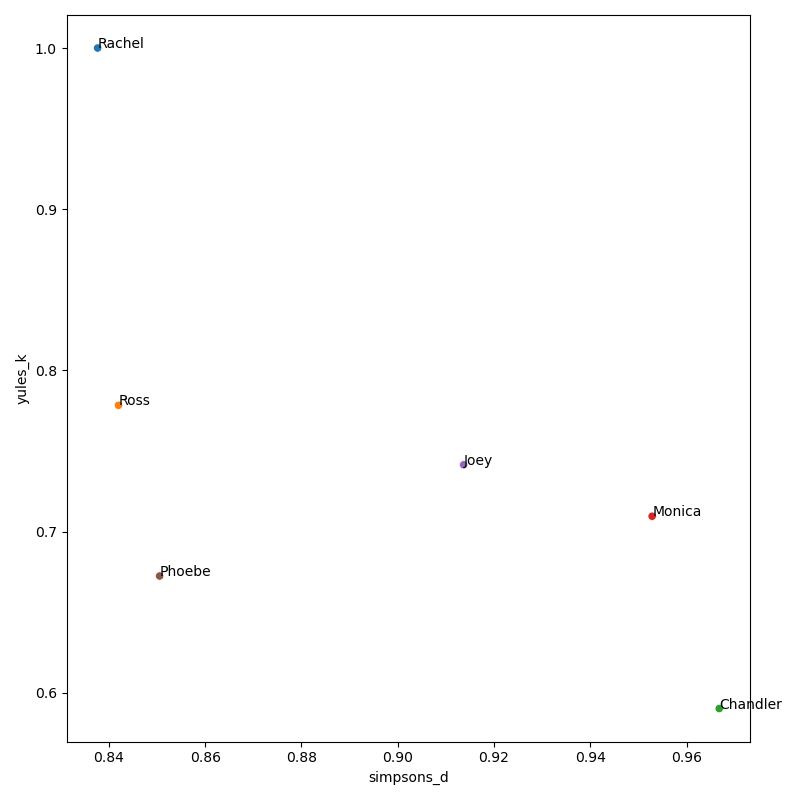
\includegraphics[width=\mediumimagewidth]{images/Friends_heuristics.png}
\end{figure}

\begin{figure}[H]
\centering
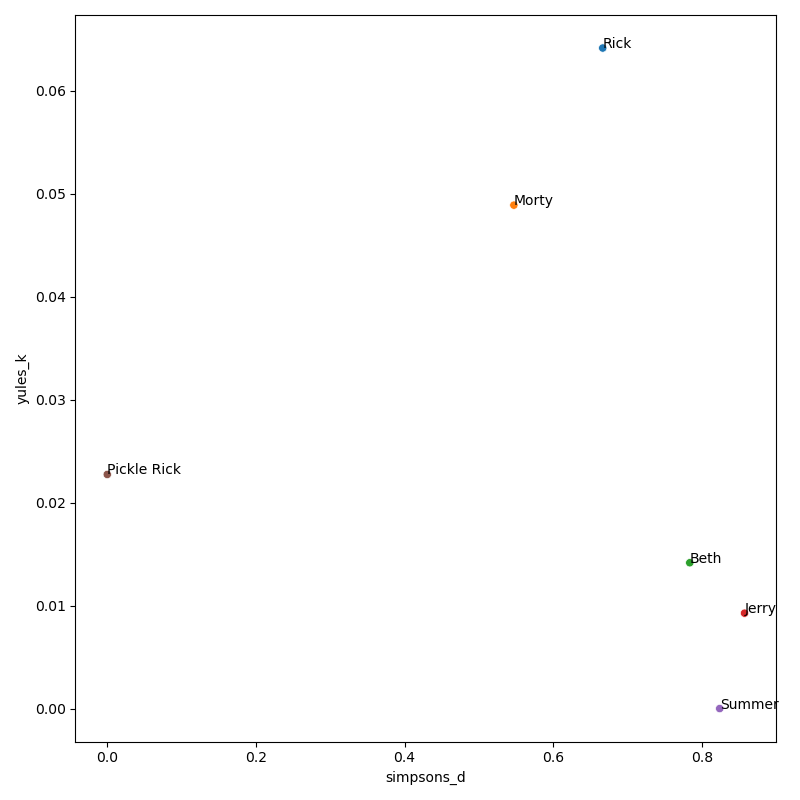
\includegraphics[width=\mediumimagewidth]{images/Rick and Morty_heuristics.png}
\end{figure}


    \begin{figure}[H]
        \centering
        \caption{Decision Stumps of AdaBoost (Misclassifications of each stump highlighted)}
        \begin{subfigure}[b]{0.45\textwidth}
            \centering
            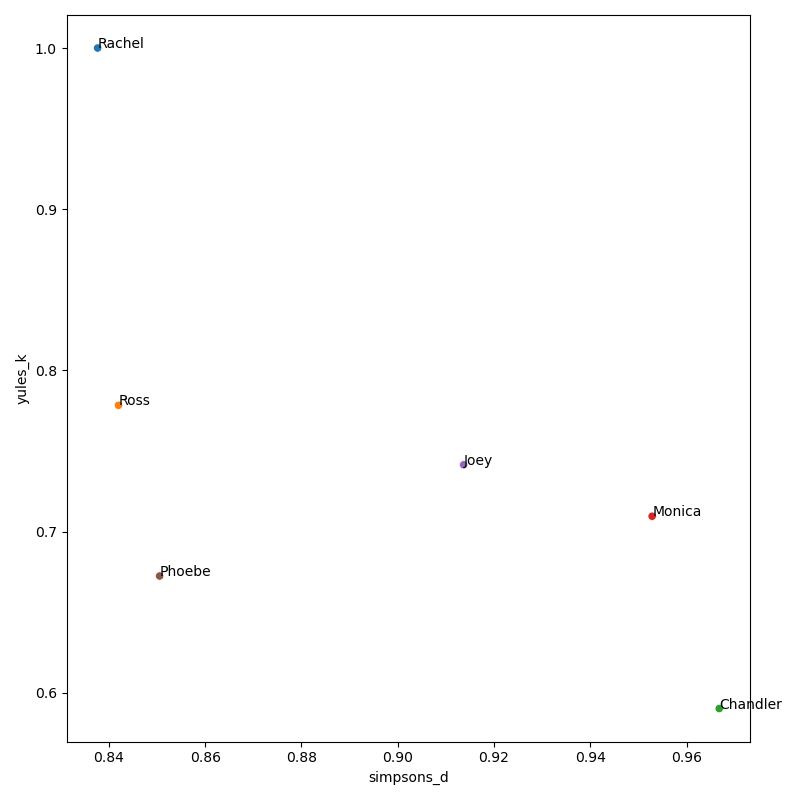
\includegraphics[width=\textwidth]{images/Friends_heuristics.png}
            \caption{T = 1}
            \label{fig:subfig1}
        \end{subfigure}
        \hfill
        \begin{subfigure}[b]{0.45\textwidth}
            \centering
            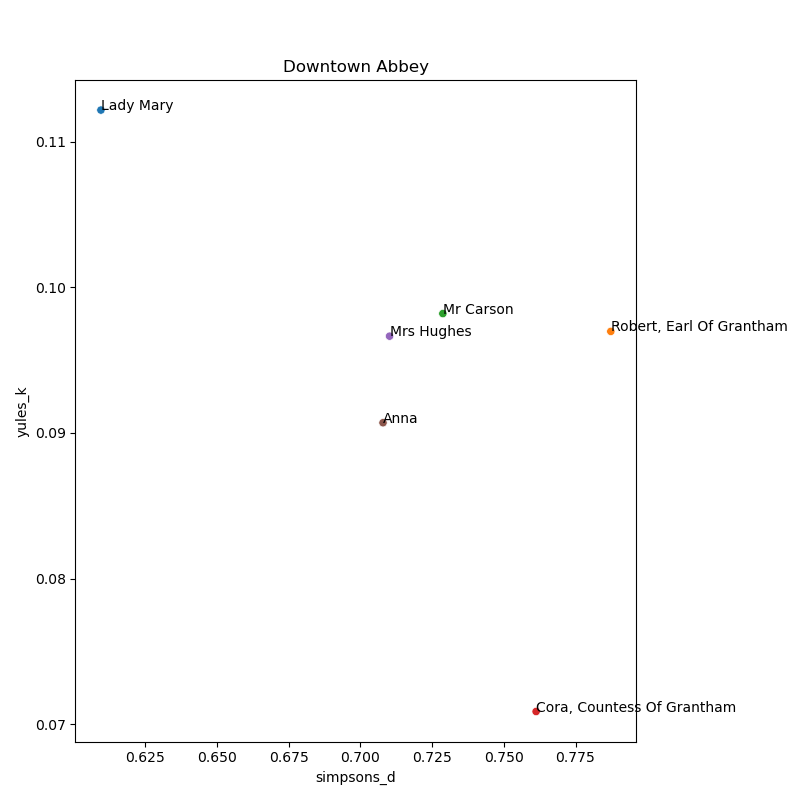
\includegraphics[width=\textwidth]{images/Downtown Abbey_heuristics.png}
            \caption{T = 2}
            \label{fig:subfig2}
        \end{subfigure}
        \label{fig:main}
    \end{figure} 
        { \Large \bfseries Project Proposal}

        \begin{itemize}
            \item[] \textbf{Problem Statement}
            
			Effective dialogue in storytelling requires that each character speak distinctly.
			The purpose of having multiple characters in a story is to provide a diversity of opinions, perspectives, and backgrounds.
			
			If every sentence spoken feels appropriate coming out of the mouth of any character, why have multiple characters at all?
			How bland would the adventures of Harry, Ron, and Hermione be if all three were equal parts courageous, loyal, and inquisitive, instead of each personality compensating for the other two?
			Would Pride and Prejudice be effective at exposing class inequalities in Victorian society if every character sounded equally posh?

			However, empirically evaluating the distinctness of each character's dialogue in a story is a subjective and challenging process. 

			This project proposes a methodology to evaluate the distinctness between sets of dialogue in terms of vocabulary, syntax, and style.
			Then, through applying this methodology to dialogue in television shows and films, assesses the ability to predict either the speaker within a show or which show among the full corpus from which the dialogue originated.
			This distinction will be referred to as $Within-Media$ and $Across-Media$ Classifications.
			
			We will conclude with a discussion of how such a model may be applied to evaluate whether the characters in a dialogue have a sufficiently unique voice. 

            \item[] \textbf{Data Sources}
            
			Fortunately, kaggle.com/datasets has data sets of dialogue with speaker labels from several well-known televison series and films:

			- \href{https://www.kaggle.com/datasets/blessondensil294/friends-tv-series-screenplay-script/data?select=S01E01+Monica+Gets+A+Roommate.txt}{Friends}: /blessondensil294/friends-tv-series-screenplay-script/
			 
			- \href{https://www.kaggle.com/datasets/pierremegret/dialogue-lines-of-the-simpsons}{The Simpsons}: /pierremegret/dialogue-lines-of-the-simpsons
			
			- \href{https://www.kaggle.com/datasets/paultimothymooney/lord-of-the-rings-data?select=lotr_scripts.csv}{The Lord of the Rings}: /paultimothymooney/lord-of-the-rings-data
			
			- \href{https://www.kaggle.com/datasets/andradaolteanu/rickmorty-scripts}{Rick and Morty}: /andradaolteanu/rickmorty-scripts

			- \href{https://scriptline.livejournal.com/71215.html#cutid6}{Pride and Prejudice, Downtown Abbey*}: scriptline.livejournal.com/71215.html
			 
			*Requires pre-processing to separate the speaker name from the dialogue spoken.

			The outcome of data pre-processing will be a corpus with the following format:
			
			\begin{table}[H]
				\centering
				\begin{tabular}{|c|c|c|}
					\hline
					\textbf{} \textbf{show} & \textbf{speaker} & \textbf{dialogue} \\
					\hline
					Friends & Phoebe &  "I asked for the news, not the weather." \\
					Friends & Phoebe &  "You'll see. You'll all see." \\
					Friends & Joey &  "How you doin'?" \\
					Pride and Prejudice & Mr. Darcy &  "My affections and wishes have not changed, but..."  \\
					The Lord of the Rings & Gollum &  "My precious!" \\
					\hline
				\end{tabular}
				\caption{Sample Rows from Dialogue Speaker Corpus}
				\label{tab:images}
			\end{table}

        \item[] \textbf{Methodology}
            
		Collect representations of dialogue that capture sufficient variability to distinguish speakers:
		
		\begin{enumerate}
			\item Heuristics
			\begin{itemize}
				\item For each speaker, calculate Yule's K and Simpson's D.
				\item Create a scatter plot to show the variability in dialogue patterns both for characters within the same piece of media and those across different pieces of media.
			\end{itemize}
		
			\item Vocabulary
			\begin{itemize}
				\item For each speaker, calculate the Term Frequency-Inverse Document Frequency (TF-IDF), where Document Frequency is based on the corpus of all dialogue of the show or film the character is present in, and store as a matrix.
				\item Include bigrams and trigrams in the matrix to capture use of multi-word expressions and catchphrases.
				\item Take the Cosine Similarity between each speaker vector with every other speaker vector in the same piece of media, plotting as a heatmap.
			\end{itemize}
		
			\item Stylometry
			\begin{itemize}
				\item For each speaker, calculate their distribution of word length and sentence length of all dialogue spoken.
				\begin{itemize}
					\item How to best represent the distribution will be a result of analyzing the distributions, although most dialogue has a skewed unimodal distribution (lots of short words and sentences, a few longer ones) that can be sufficiently captured by mean, standard deviation, and skewness.
				\end{itemize}
				\item For each speaker, calculate the frequency of their use of function words and common punctuation, again plotting Cosine Similarity as a heatmap.
			\end{itemize}
		
			\item Visualize
			\begin{itemize}
				\item Create a scatter plot showing the Cosine Similarity of the Vocabulary Matrix on one axis and stylometry on the other.
				\begin{itemize}
					\item Generate Heatmaps that use different measures of distance (Manhattan, Euclidean, etc.) and consider pros and cons of adopting them as alternatives.
				\end{itemize}
			\end{itemize}
		\end{enumerate}
	
		\item[] \textbf{Evaluation}

		Within-Media

		\begin{enumerate}
			\item For each media (i.e. movie or show), train a Naive Bayes classifier on the Vocabulary and Stylometry matrices.
			\item Interpret the results. Which media has dialogue that the Bayesian Classifier can most effectively predict?
		\end{enumerate}

		Across-Media

		\begin{enumerate}
			\item Perform PCA on the TF-IDF vectors that represent each speaker with each media.
			\item Perform K-means Clustering on the top 2-3 components of the resulting dataset, where $k$ equals the number of distinct tv shows and movies. Calculate the purity score where ``each cluster is assigned to the class which is most frequent in the cluster'' (taken verbatim from HW1).
			\item Interpret the results. Which clusters have the highest and lowest purity scores?
		\end{enumerate}
		

\item[] \textbf{Applications of Coursework}

- \textbf{Naive Bayes} to train a classifier to predict a speaker within a specific piece of media

- \textbf{Minkowski Distances} (Euclidean, Manhattan, etc)

- \textbf{Principal Component Analysis} to prepare TF-IDF vectors for clustering

- \textbf{K-Means Clustering} to classify speakers of dialogue across media

\item[] \textbf{Background}

Can, F., and Patton, J. M. (2004). Change of Writing Style with Time. Computers and the Humanities, 38(1), 61 82. http://www.jstor.org/stable/30204925

Kumiko Tanaka-Ishii, Shunsuke Aihara; Computational Constancy Measures of Texts—Yule's K and Rényi's Entropy. Computational Linguistics 2015; 41 (3): 481 502. Link.

Simpson, E. Measurement of Diversity. Nature 163, 688 (1949). Link. 

Spärck Jones, K. (2021). A statistical interpretation of term specificity and its application in retrieval. J. Documentation, 60, 493-502.

Tweedie, F. J., Singh, S., and Holmes, D. I. (1996). Neural Network Applications in Stylometry: The “Federalist Papers.” Computers and the Humanities, 30(1), 1 10. http://www.jstor.org/stable/30204514
   

    \end{itemize}
	
	\pagebreak

\end{titlepage}


\end{document}

